\documentclass[9pt, aspectratio=169]{beamer}
\mode<presentation>
\usepackage[T1]{fontenc}
\usepackage{color}
\usepackage{graphicx}
\usepackage{natbib}
\usepackage{tikz}
\usepackage{booktabs}
\usepackage{tcolorbox}

\usetheme{Boadilla}


\definecolor{mcctext}{HTML}{0d77b0}
\definecolor{mcclogo}{HTML}{0067a1}
\definecolor{mcclight}{HTML}{D9E8F1}


\usecolortheme[named=mcclogo]{structure}


\usefonttheme{professionalfonts}

\newtheorem*{remark}{}

\bibliographystyle{apalike}

\title[Stopping Criteria]{Statistical Stopping Criteria for Automated Screening in Systematic Reviews}
\subtitle{}
\author{Max Callaghan, Finn Müller-Hansen }
\institute[MCC]{
	
\includegraphics[height=1cm,width=2cm]{images/MCC_Logo_RZ_rgb.jpg} \hspace{3em}
	
\includegraphics[height=1cm]{images/University-of-Leeds-logo.png}
}
\date{September 26, 2019}

\begin{document}
	
\setbeamertemplate{caption}{\raggedright\insertcaption\par}
	
	\begin{frame}
	\titlepage
\end{frame}

\begin{frame}{Context - the promise of work savings through machine learning}

\begin{columns}
	\begin{column}{0.618\linewidth}
		\begin{itemize}
			\item When doing a systematic review, or other evidence synthesis project, you often need to screen a lot of documents.
			\item Large literature on training machine learning algorithms to recognise relevant documents and give these to us first \cite{OMara-Eves2015}.
			\item The promise of this field is that we can stop before screening all documents, saving humans work.
		\end{itemize}
	
		\medskip	
			
		\textbf{But,}
		

		\begin{itemize}
			\item How do we know what a good time to stop is?
			\item How can we report this?
		\end{itemize}
		
		
		
		
	\end{column}
	\begin{column}{0.382\linewidth}
		\begin{figure}
			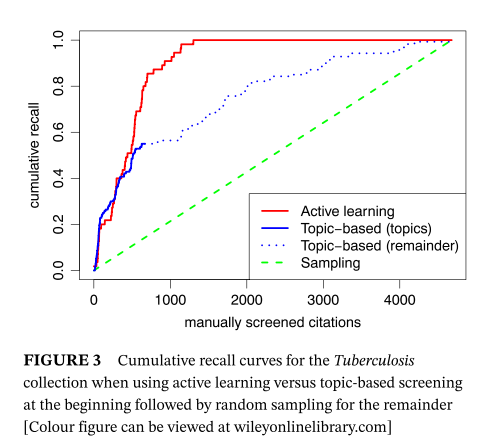
\includegraphics[width=\linewidth]{images/example-recall}
			\caption{Source: \cite{Przybya2018}}
		\end{figure}
	\end{column}
\end{columns}

\end{frame}

\begin{frame}{Workflows for reducing human effort in systematic review screening}

\begin{columns}
	\begin{column}{0.6\linewidth}
		\begin{figure}
			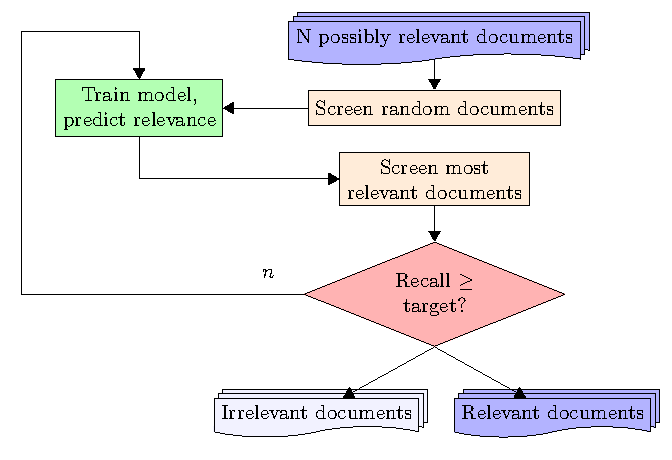
\includegraphics[width=\linewidth]{../images/flow_noeq_basic.pdf}
		\end{figure}
	\end{column}
	\begin{column}{0.4\linewidth}
		Existing approaches to deciding when to stop screening are unsatisfactory \cite{bannach-brown2019, Marshall2019}, but fall into the following categories
		
		\medskip
		
		\begin{itemize}
			\item \textbf{BIR Sampling:} Estimate the number of relevant documents via sampling, stop when you have seen that number \cite{Shemilt2014}
			\item \textbf{Heuristics:} Stop after [x] consecutive irrelevant documents \cite{Jonnalagadda2013, Przybya2018}
			\item \textbf{Novel automatic stopping criteria:} More sophisticated systems for automatically deciding when to stop screening \cite{Yu2019, DiNunzio2018, Howard2020}
		\end{itemize}
		
	\end{column}
\end{columns}

\end{frame}

\begin{frame}{Baseline Inclusion Rate (BIR) Sampling based criteria}
\begin{columns}
	\begin{column}{0.382\linewidth}
		\begin{enumerate}
			\item Sample a fraction of large set of documents
			\item Estimate the number of relevant documents based on the number seen in the sample
			\item Screen until this number of relevant documents (or a proportion corresponding to target recall) has been seen.
		\end{enumerate}
	
		\begin{remark}
			Sampling error is not accounted for and can have serious consequences
		\end{remark}
	\end{column}
	\begin{column}{0.618\linewidth}
		\begin{figure}
		\only<1>{
		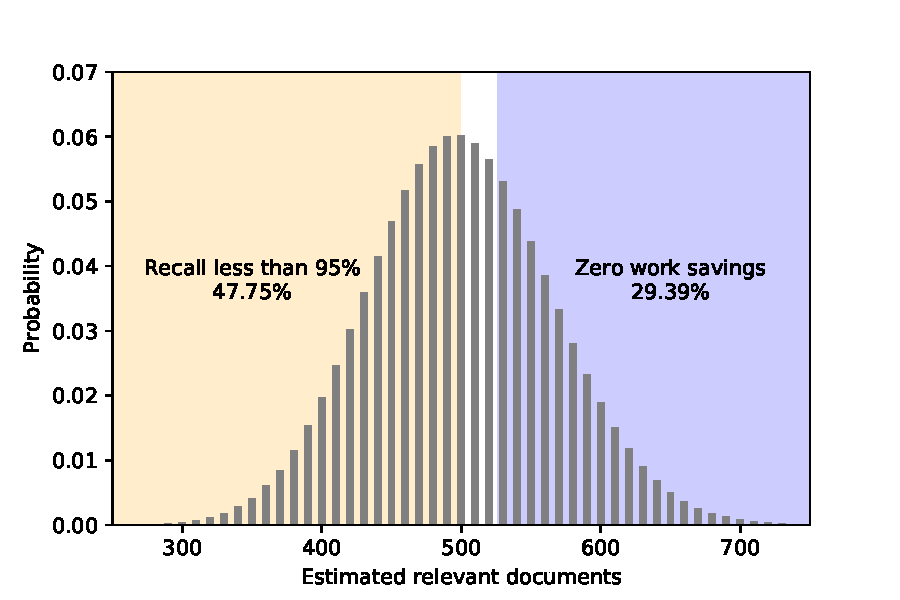
\includegraphics[width=\linewidth]{../manuscript/2_figs_bir_errors.pdf}
		\caption{\small Distribution of errors after a sample of 1,000 using the BIR sampling method in a dataset of 20,000 documents of which 500 are relevant. }}
		\only<2>{
	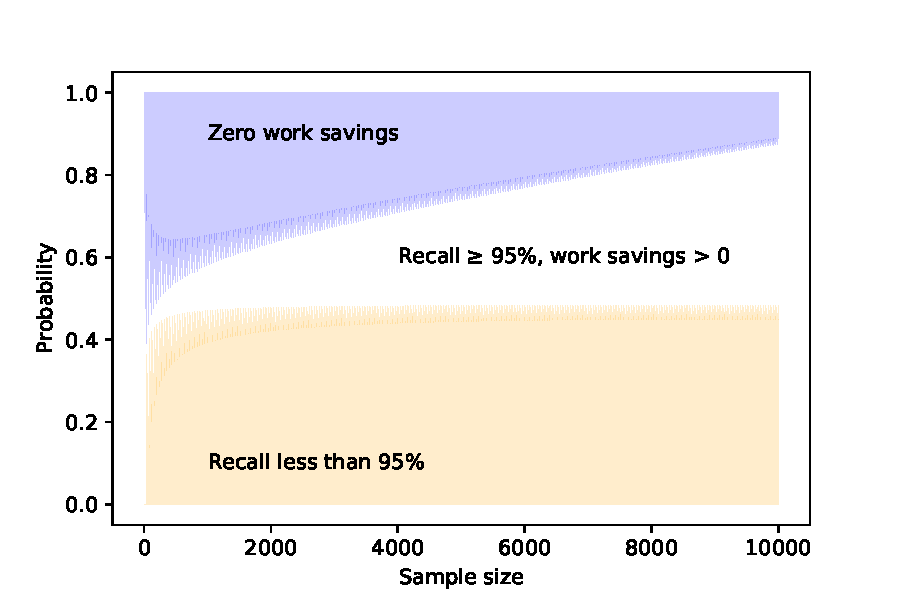
\includegraphics[width=\linewidth]{../manuscript/2_figs_bir_error_distribution.pdf}
	\caption{\small Distribution of errors across sample sizes using the BIR sampling method in a dataset of 20,000 documents of which 500 are relevant. }}
		\end{figure}


	\end{column}
\end{columns}
\end{frame}

\begin{frame}{Heuristic criteria}
\begin{columns}
	\begin{column}{0.618\linewidth}
		\begin{itemize}
			\item If we see several consecutive irrelevant documents, we can surmise that the proportion of relevant documents remaining is low
		\end{itemize}
	
		\begin{remark}<2->
			This intuition is helpful, but misses the fact that the proportion of relevant documents in the set of unseen documents can mean very different things
		\end{remark}
	\end{column}
	\begin{column}{0.382\linewidth}
		
		\begin{figure}
			\only<1->{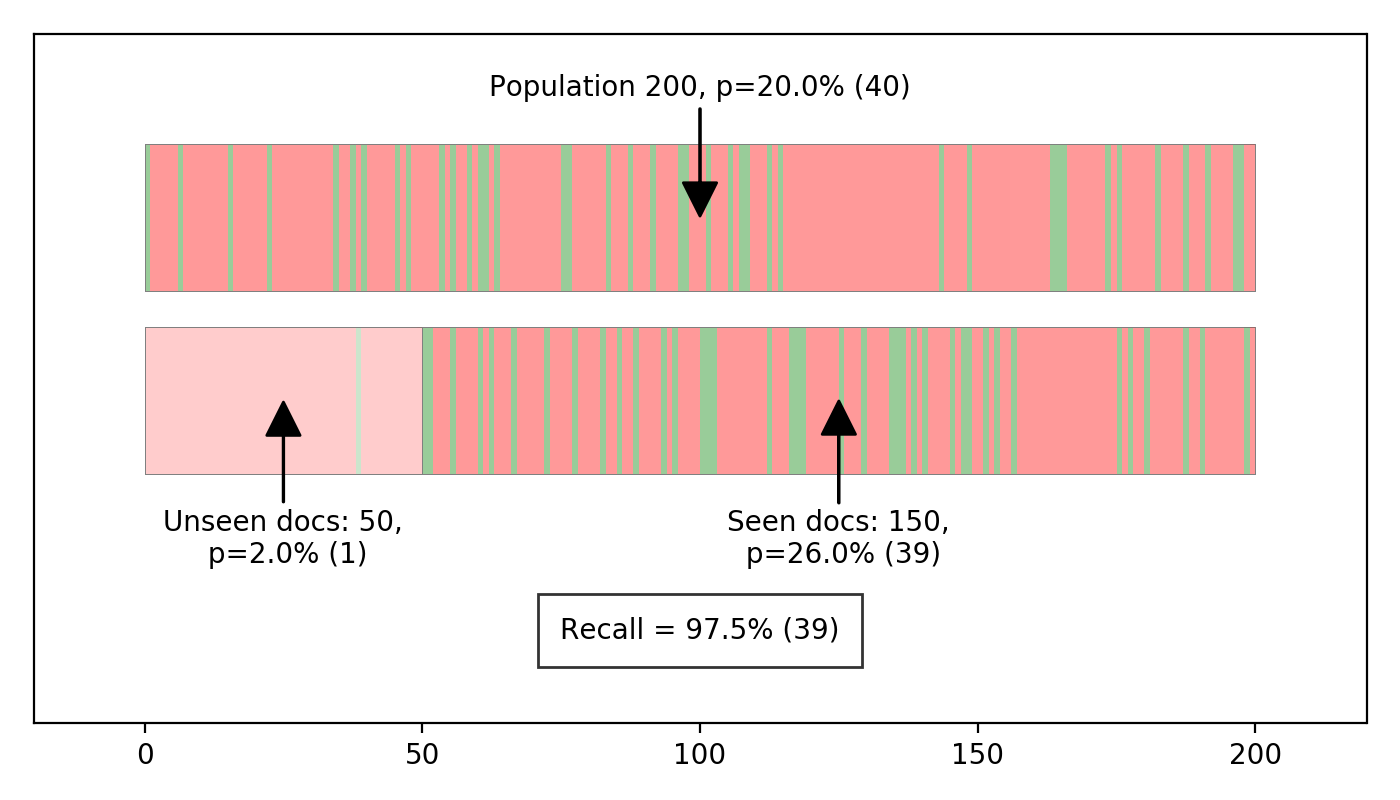
\includegraphics[width=\linewidth]{../manuscript/2_figs_proportions_2}}
			\only<2->{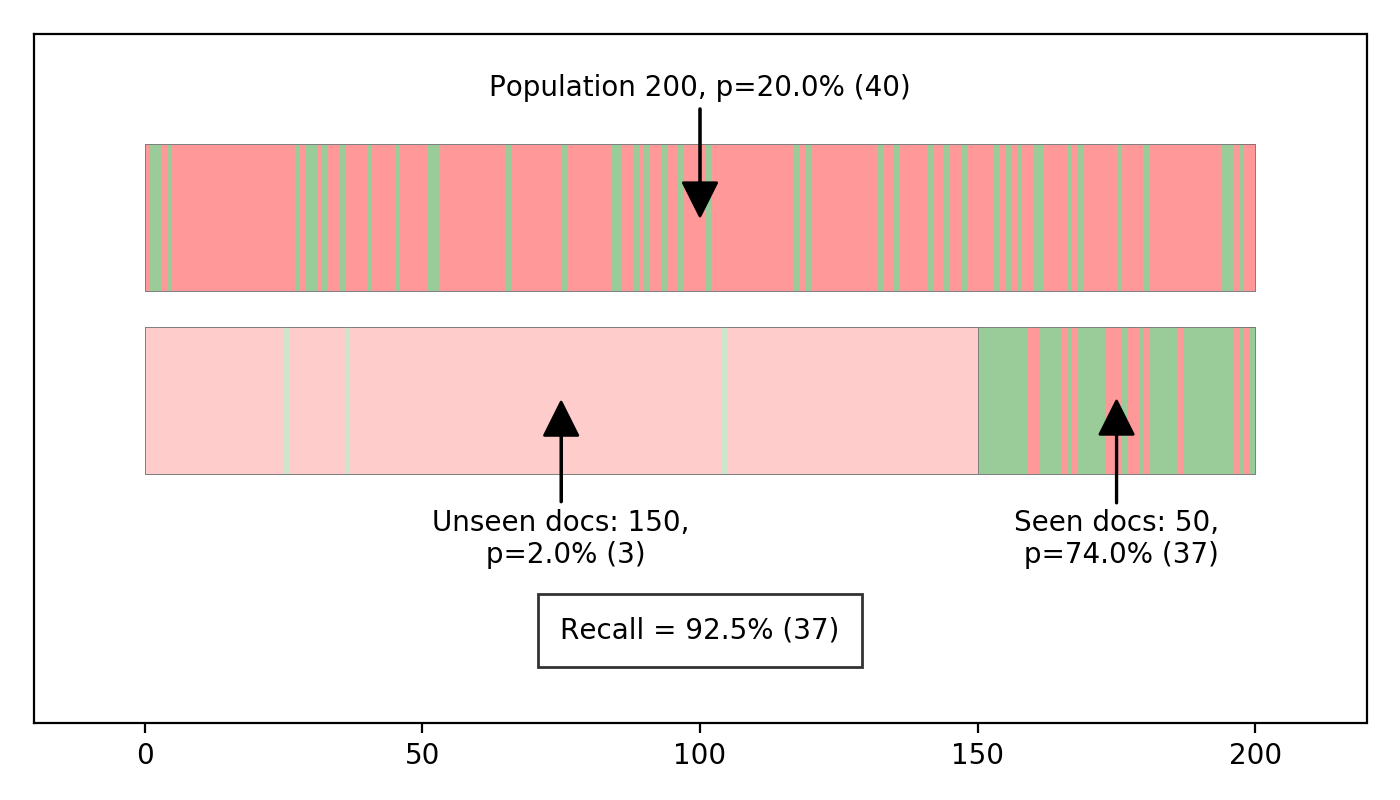
\includegraphics[width=\linewidth]{../manuscript/2_figs_proportions_1}}
		\end{figure}

	\end{column}
\end{columns}
\end{frame}

\begin{frame}{Novel automatic stopping criteria}

Several recent papers \cite{Yu2019, DiNunzio2018, Howard2020} have suggested more sophisticated stopping criteria.

\medskip

None of these have the same \textit{fundamental} problems as those discussed, but

\begin{itemize}
	\item None account properly for uncertainty
	\item None deliver \textit{reliable} meeting of recall targets
	\item None offer users the ability to communicate when they stopped
\end{itemize}

\begin{remark}
	If we want to use machine learning in live systematic reviews, we need criteria that can communicate the probable outcome of stopping early in a way that is clear and independent of machine learning approach and performance
\end{remark}

\end{frame}


\begin{frame}{A statistical stopping criteria for Active Learning}

We test a null hypothesis that a given recall target has not been achieved, starting a random sample at an arbitrary point. 

\textbf{Definitions}

\begin{itemize}
	\item $N_{tot}$ is the total number of documents
	\item $\rho_{tot}$ is the total number of relevant documents
	\item $\rho_{seen}$ is the number of relevant documents seen by a screener
	\item $\tau$, or recall is $\frac{\rho_{seen}}{\rho_{tot}}$
	\item $\tau_{tar}$ is our recall target
	\item $N_{AL}$ is the number of documents seen after active learning has finished (at start of random sample)
	\item $N$ is the number of documents in the sample ($N_{tot} - N_{AL}$)
	\item $K$ is the number of relevant documents in the sample ($\rho_{tot} - \rho_{AL}$)
\end{itemize}

After each draw from the sample:

\begin{itemize}
	\item $n$ is the number of documents drawn
	\item $k$ is the number of relevant drawn
\end{itemize}

\end{frame}

\begin{frame}{A statistical stopping criteria for Active Learning - II}

We form a null hypothesis that the target recall has not been achieved

\begin{equation}
H_0 : \tau < \tau_{tar}
\label{eq:null_hypothesis}
\end{equation}

Accordingly, our alternative hypothesis is that recall is at least as large as our target:

\begin{equation}
H_1 : \tau \geq \tau_{tar}
\end{equation}

Because we are sampling without replacement, we know that $k$ is distributed hypergeometrically:

\begin{equation}
k \sim Hypergeometric(N, K, n)
\end{equation}

\end{frame}


\begin{frame}{A statistical stopping criteria for Active Learning - III}

		
We introduce a hypothetical value for $K$, which we call $K_{tar}$. This represents the lowest value for $K$ compatible with $H_0$

\begin{equation}
K_{tar} = \lfloor \frac{\rho_{seen}}{\tau_{tar}}-\rho_{AL}+1 \rfloor
\end{equation}

An testable analogue of $H_0$ is therefore

\begin{equation}
H_0 : K \geq K_{tar}
\end{equation}

The cumulative distribution function gives us the probability of observing what we observed, if our null hypothesis were true

\begin{equation}
p = P(X \leq k) \text{, where } X \sim Hypergeometric(N,K_{tar},n)
\label{eq:p-value}
\end{equation}

When $p < 1-\alpha$, we can stop screening, and report, for example, that we reject the null hypothesis that we achieve a recall below 95\% at the 5\% significance level

\end{frame}

\begin{frame}{A statistical stopping criteria for active learning - When to start a random sample?}

\begin{columns}
	\begin{column}{0.382\linewidth}
		\begin{figure}
			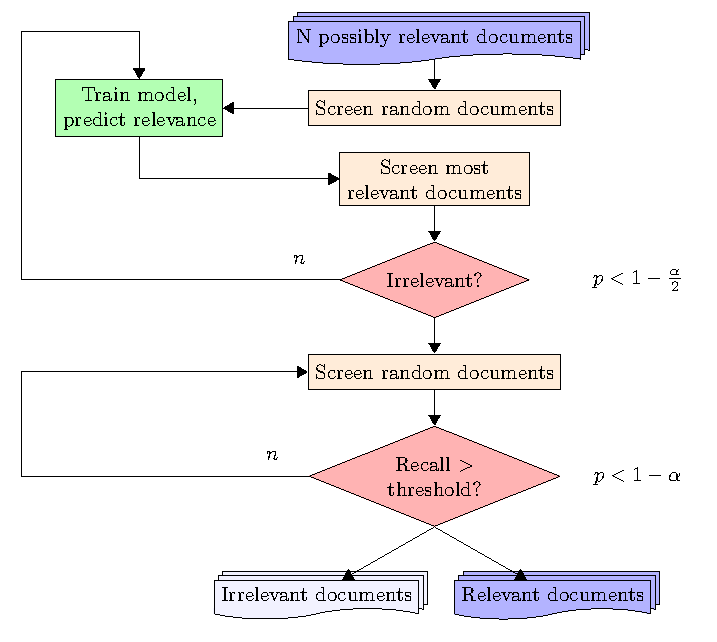
\includegraphics[width=\linewidth]{../images/flow.pdf}
		\end{figure}
	\end{column}
	\begin{column}{0.618\linewidth}
		In the approach described, we need to stop machine learning at some point and switch to random sampling
		\begin{itemize}
			\item If we stop too early, it will take us a long time to get to our recall target
			\item If we stop too late, we will save less work
		\end{itemize}
	
		\medskip
	
		We define a subcriterion, ``ranked quasi-sampling'', which treats previously screened documents as random samples.
		
		\begin{itemize}
			\item Ranked quasi-sampling is always conservative, as long as the proportion of relevant documents given to the screener by the machine learning algorithm $\geq$ the proportion in the remaining documents
			\item We test this as an independent criteria, but also use it to decide when to stop screening
		\end{itemize}
	\end{column}
\end{columns}

\end{frame}

\begin{frame}{Evaluation}
\begin{columns}
	\begin{column}{0.618\linewidth}
		\begin{table}
			\footnotesize
			\begin{tabular}{lllrrr}
\toprule
{} &                  dataset & data\_source &     N &  r\_docs &    p \\
\midrule
0  &      UrinaryIncontinence &       cohen &   284 &      68 & 0.24 \\
1  &           Antihistamines &       cohen &   287 &      90 & 0.31 \\
2  &                Estrogens &       cohen &   349 &      79 & 0.23 \\
3  &                   NSAIDS &       cohen &   358 &      83 & 0.23 \\
4  &        OralHypoglycemics &       cohen &   475 &     135 & 0.28 \\
5  &                 Triptans &       cohen &   594 &     205 & 0.35 \\
6  &                     ADHD &       cohen &   803 &      83 & 0.10 \\
7  &   AtypicalAntipsychotics &       cohen &  1030 &     333 & 0.32 \\
8  &   CalciumChannelBlockers &       cohen &  1103 &     257 & 0.23 \\
9  &     ProtonPumpInhibitors &       cohen &  1210 &     227 & 0.19 \\
10 &  SkeletalMuscleRelaxants &       cohen &  1348 &      30 & 0.02 \\
11 &                     COPD &     copd\_pb &  1443 &     179 & 0.12 \\
12 &               Kitchenham &    fastread &  1700 &      45 & 0.03 \\
13 &                   Opiods &       cohen &  1769 &      43 & 0.02 \\
14 &             BetaBlockers &       cohen &  1872 &     270 & 0.14 \\
15 &            ACEInhibitors &       cohen &  2234 &     168 & 0.08 \\
16 &                  Statins &       cohen &  2743 &     152 & 0.06 \\
17 &               ProtonBeam &     copd\_pb &  4108 &     240 & 0.06 \\
18 &               Radjenovic &    fastread &  5999 &      47 & 0.01 \\
19 &                   Wahono &    fastread &  7002 &      62 & 0.01 \\
20 &                     Hall &    fastread &  8911 &     104 & 0.01 \\
\bottomrule
\end{tabular}

			\caption{Dataset properties}
			\label{tab:data}
		\end{table}
	\end{column}
	\begin{column}{0.382\linewidth}
		
		\begin{itemize}
			\item We assemble a dataset of systematic reviews which other systems have been tested on
			\item We simulate 100 reviews on each of these
			\item In each review, a sample is drawn to begin with, then every 10 documents:
			\begin{itemize}
				\item a simple SVM is trained on documents already seen
				\item the relevance of unseen documents is predicted
				\item the real relevance values of the next 10 documents are revealed
			\end{itemize}
			\item We record when each criteria would have been achieved
		\end{itemize}
		
	\end{column}
\end{columns}

\end{frame}

\begin{frame}{Criteria performance - A priori knowledge}

\begin{columns}
	\begin{column}{0.5\linewidth}
		\begin{figure}
			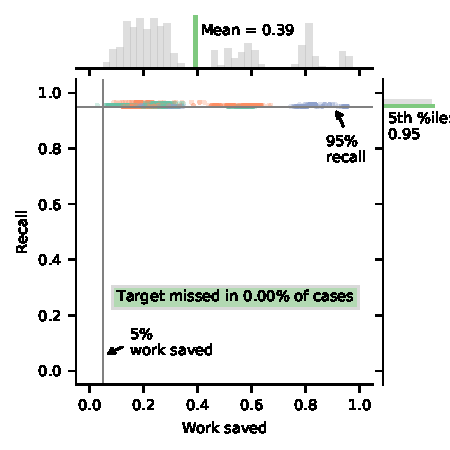
\includegraphics[width=\linewidth]{../manuscript/2_figs_jointplot_pf.pdf}

		\end{figure}
	\end{column}
	\begin{column}{0.5\linewidth}
		This is what would happen if we already knew how many relevant documents there were.
			
			\medskip 
			
			The target is never missed, and we can achieve some very large work savings.
			
			\medskip
			
			These are the results most often reported!

	\end{column}
\end{columns}
\end{frame}


\begin{frame}{Criteria performance - Baseline estimation}

\begin{columns}
	\begin{column}{0.5\linewidth}
		\begin{figure}
			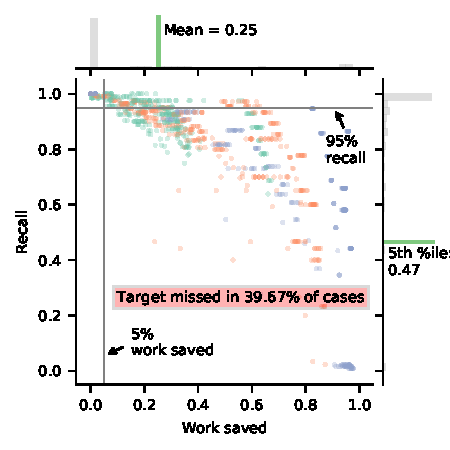
\includegraphics[width=\linewidth]{../manuscript/2_figs_jointplot_bir.pdf}
		\end{figure}
	\end{column}
	\begin{column}{0.5\linewidth}
Estimating the number of relevant results based on a sample means we often (drastically!) miss our target, and we often save no work at all
		
	\end{column}
\end{columns}

\end{frame}



\begin{frame}{Criteria performance - Heuristics}

\begin{columns}
	\begin{column}{0.5\linewidth}
		\begin{figure}
			\only<1>{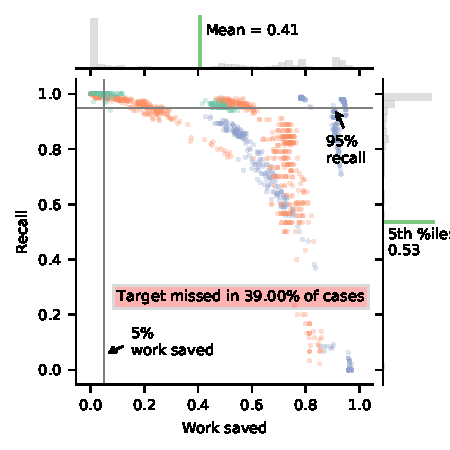
\includegraphics[width=\linewidth]{../manuscript/2_figs_jointplot_ih_50.pdf}}
			\only<2>{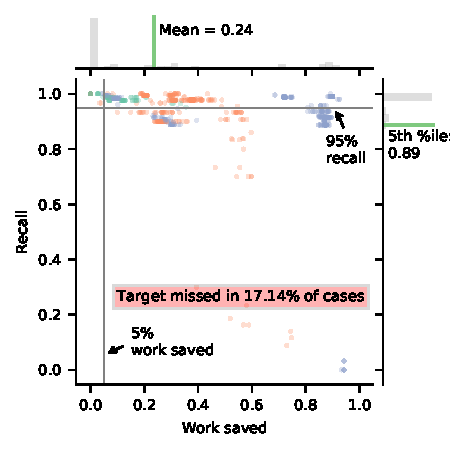
\includegraphics[width=\linewidth]{../manuscript/2_figs_jointplot_ih_200.pdf}}
		\end{figure}
	\end{column}
	\begin{column}{0.5\linewidth}
		\only<1-2>{Stopping after 50 consecutive irrelevant results sometimes works, but often results in awful recall or no work savings}
		\only<2>{
			\medskip
			
			A stricter heuristic (200 consecutive irrelevant results) less often leads to poor recall, but also means less work is saved)
		}
	\end{column}
\end{columns}

\end{frame}


\begin{frame}{Criteria performance - Statistical stopping criteria (random sampling)}

\begin{columns}
	\begin{column}{0.5\linewidth}
		\begin{figure}
			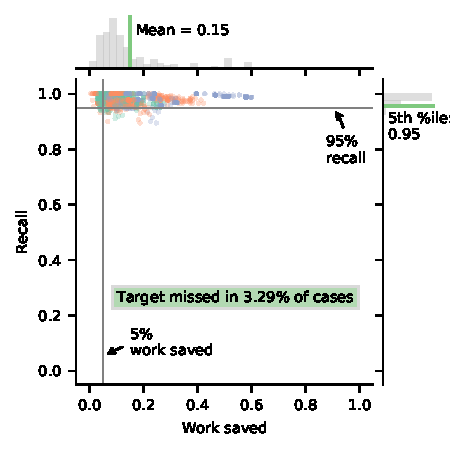
\includegraphics[width=\linewidth]{../manuscript/2_figs_jointplot_hyper.pdf}
			
		\end{figure}
	\end{column}
	\begin{column}{0.5\linewidth}
		Our basic criterion makes modest work savings possible with a reliable achievement of the recall target
		
	\end{column}
\end{columns}

\end{frame}

\begin{frame}{Criteria performance - Statistical stopping criteria (ranked quasi-random sampling)}

\begin{columns}
	\begin{column}{0.5\linewidth}
		\begin{figure}
			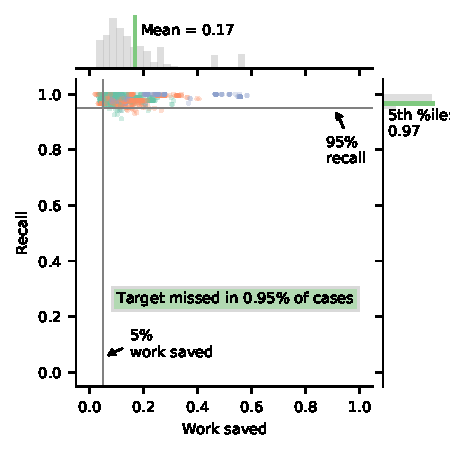
\includegraphics[width=\linewidth]{../manuscript/2_figs_jointplot_nrs.pdf}
			
		\end{figure}
	\end{column}
	\begin{column}{0.5\linewidth}
		Our criterion using ranked quasi-sampling turns out to be more conservative, and to allow slightly larger work savings, but this is not robust to catastrophic machine learning failure!
		
	\end{column}
\end{columns}

\end{frame}

\begin{frame}{Discussion}

\begin{columns}
	\begin{column}{0.618\linewidth}
		 \begin{itemize}
		 	\item We provide reliable stopping criteria that realise \textit{some} of the work savings in systematic review screening promised by machine learning
		 	\item Previously the outcome of a badly performing machine learning model could have been low recall levels (as low as a few percent). Now only work savings are at risk.
		 	\item We can use these in live reviews, because we can report the implications of our decision to stop early for recall
		 \end{itemize}
	\end{column}
	\begin{column}{0.382\linewidth}
		Work savings are modest but
		\begin{itemize}
			\item We used very general machine learning models and did not tune the parameters to perform better on individual datasets
			\item Larger savings are possible in larger datasets (where work savings are most helpful!)
			\item Forthcoming work will investigate how work savings depend on data features -> savings calculator for new projects
		\end{itemize}
	\end{column}
\end{columns}

\begin{center}
	\line(1,0){250}
	
	\medskip
	
	\textbf{Thanks!}
	
	\medskip
	
	Working paper: \url{https://doi.org/10.21203/rs.2.18218/v2}
	
	Contact: \url{callaghan@mcc-berlin.net}, Twitter: @MaxCallaghan5
	
	Code: \url{https://github.com/mcallaghan/rapid-screening}
	
\end{center}

\end{frame}


\begin{frame}{References}
\tiny
\bibliography{../manuscript/3_bib_mendeley}
\end{frame}

\end{document}